\documentclass[a4paper, 12pt]{article}

\usepackage{graphicx}
\graphicspath{ {./img/} }
\usepackage[hidelinks]{hyperref}

\newcommand{\projectname}{CT4101 Report - Cedar Pfeiffer 23701881}

\setlength\parindent{0pt}

\usepackage{fancyhdr}
\setlength{\headheight}{15.2pt}
\pagestyle{fancy}
\fancyhf{}
\renewcommand{\headrulewidth}{0px}

\fancyhead[L]{\projectname}
\fancyfoot[R]{\thepage}

\begin{document}

\pagenumbering{arabic}
\fancyfoot[R]{Page \thepage}

\begin{titlepage}
    \centering
    \vspace*{4cm}
    {\Large Final Report  \par}
    \vspace{0.5cm}
    {\Large Version 1.0 \par}
    \vspace{0.5cm}
    {\Large \today \par}
    \vspace{2cm}
    {\Large Cedar Pfeiffer (23701881)\par}
    \vfill

    Prepared for\\
    CT4101--Machine Learning\par

\end{titlepage}

\newpage 

\tableofcontents

\newpage


\section{Introduction}
This is the final report for the CT417 Machine Learning module portfolio assignment.
This report will cover an analysis of the dataset used, models chosen, preprocessing done, tuning performed, error analysis on each model and a final result.\\
The chosen task for this portfolio is regression on the dataset abalone\cite{abalone}, which records various physical measurements of abalone with the goal of predicting the age of a given specimen. Abalone are sea snails used as a food source and as a material to create jewllery or other decorative items.\\
The repository for this project can be found \underline{\href{https://github.com/queersweetpotato/machine-learning}{here}}. Its structure and any required run instructions or packages are explained in the repository. It consists of a readme explaining the project, a requirements.txt listing all needed packages, and a notebooks directory with independent jupyter notebooks containing the anaylsis and work done.\\
The report is accompanied by a video explaining the repository and outcomes, which has been uploaded on canvas.

\section{Assistance Declaration}

I hereby declare that I used no assistance from AI, coding assistants, human collaborators or used any external code anywhere in the repository, this report,  or for the video submitted as part of this assigment. 
This includes this report, the video, all notebooks, and instructions in the readme and requirements.txt, as well as any ideas and analysis. 
All outside sources used are cited in the bibliography below.

\section{Dataset Chosen}
The dataset used is Abalone\cite{abalone}, assembled by Nash et al in 1994.
This dataset is licensed under a Creative Commons Attribution 4.0 International (CC BY 4.0) license, which means it is free to use so long as it has been properly cited.\\
It has already undergone preprocessing by Nash et al, who scaled the ranges of all continuous variables by dividing by 200.\\

As mentioned above, it is a dataset for a regression task to predict the age of an abalone. 
A given specimen's age can be measured by staining and counting its rings, but this is a time consuming process and prone to human error. Thus it would be pratical to be able to predict the age without needing to do it manually. If it were possible to do it without needing to dissect the abalone, this could also be very useful.\\  

The dataset has 4177 features, 8 input variables and one target. The inputs are sex, length, diameter, height, whole weight, shucked weight, viscera weigh, and shell weight and the target is rings (translates into age by adding 1.5).
Details can be seen in the table below.\vspace{0.5cm}\\
\begin{tabular}{ |c|c|c|c|c|} 
\hline
          name  &   role &        type  & description                & units   \\
\hline
          Sex & Feature &  Categorical & M, F, and I (infant)       & NaN         \\
\hline 
        Length & Feature &  Continuous  & Longest shell measurement  & mm         \\  
\hline
      Diameter & Feature &  Continuous  & Perpendicular to length    & mm           \\
\hline      
  Height & Feature &  Continuous        & With meat in shell         & mm      \\ 
\hline  
Whole\_weight& Feature &  Continuous   & Whole weight               & grams   \\   
\hline
Shucked\_weight& Feature &  Continuous  & Weight of meat             & grams    \\   
\hline
Viscera\_weight& Feature &  Continuous  & Gut weight (after bleeding)& grams    \\   
\hline  
Shell\_weight& Feature &  Continuous    & After being dried          & grams   \\   
\hline         
Rings & Target  &  Integer              & +1.5 gives the age in years& NaN           \\
\hline   

\end{tabular}

There are no missing variables, and no duplicates among the instances. All of features will be available to the model at prediction time, as they are measurements that can be taken from an abalone simultaneously.
There are no dependencies between different features, as each row covers the measurements of a separate abalone.

Some outliers can be visually detected by examining the histograms generated in the dataset notebook, and their specific data can be read in the listings of the three largest and smalles rows for each column (also in the dataset notebook). 
For example, feature 236 is the the smallest in all variables but height. This is because it is the youngest abalone in the dataset, with only one ring.
All outliers detected seem to be rare, valid cases (e.g. the smallest values are very young specimens), so there is no need to remove them.
From looking at the outliers we can also see that the data is not completely linear, as the oldest specimen (feature 480 at 29 rings) is not the largest in any category (that honour being spread across features 1428, 2051, 891, 1209, and 1763, none of which are in the top three oldest specimens).\\
Below some selected histograms are shown. One can see that sex is roughly evenly distributed, and some outliers in the whole\_weight variable.

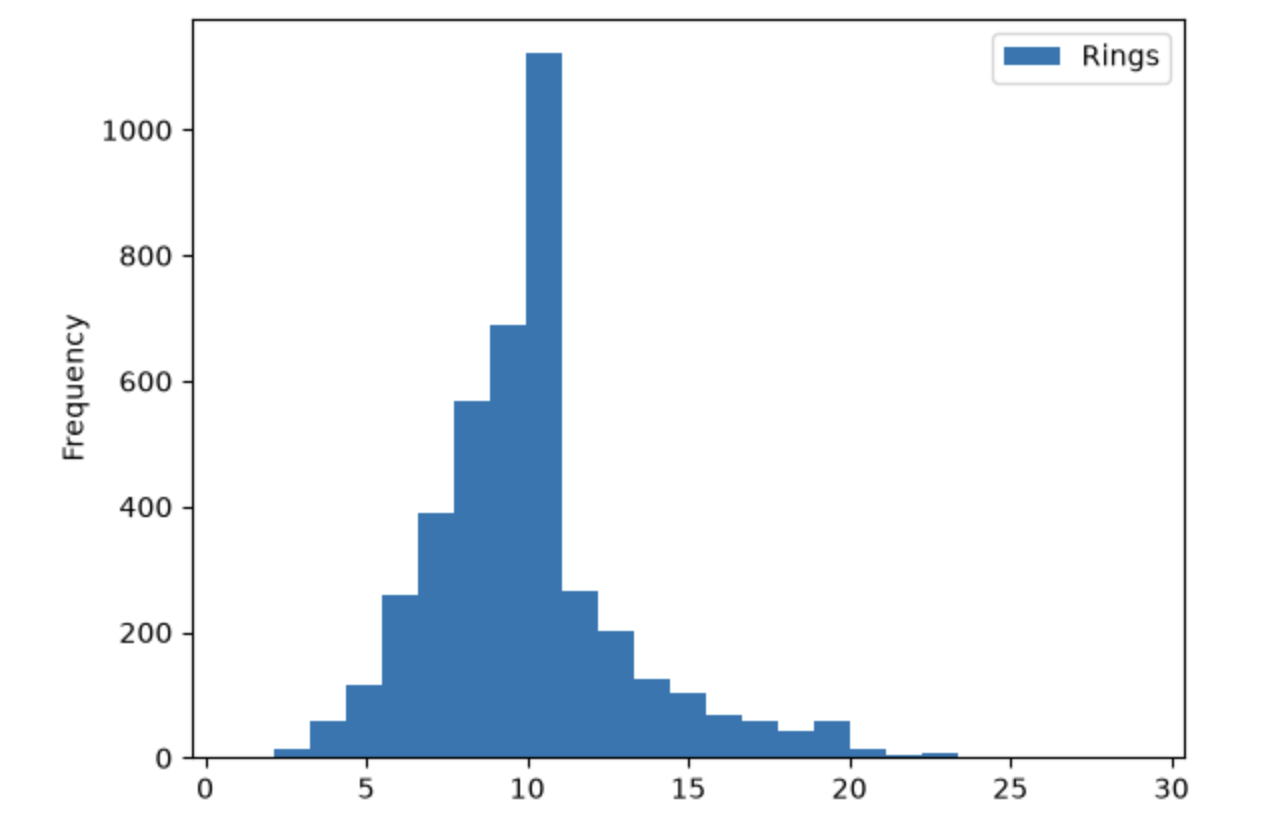
\includegraphics[width=10cm]{target_distribution.png}\\
Target Distribution

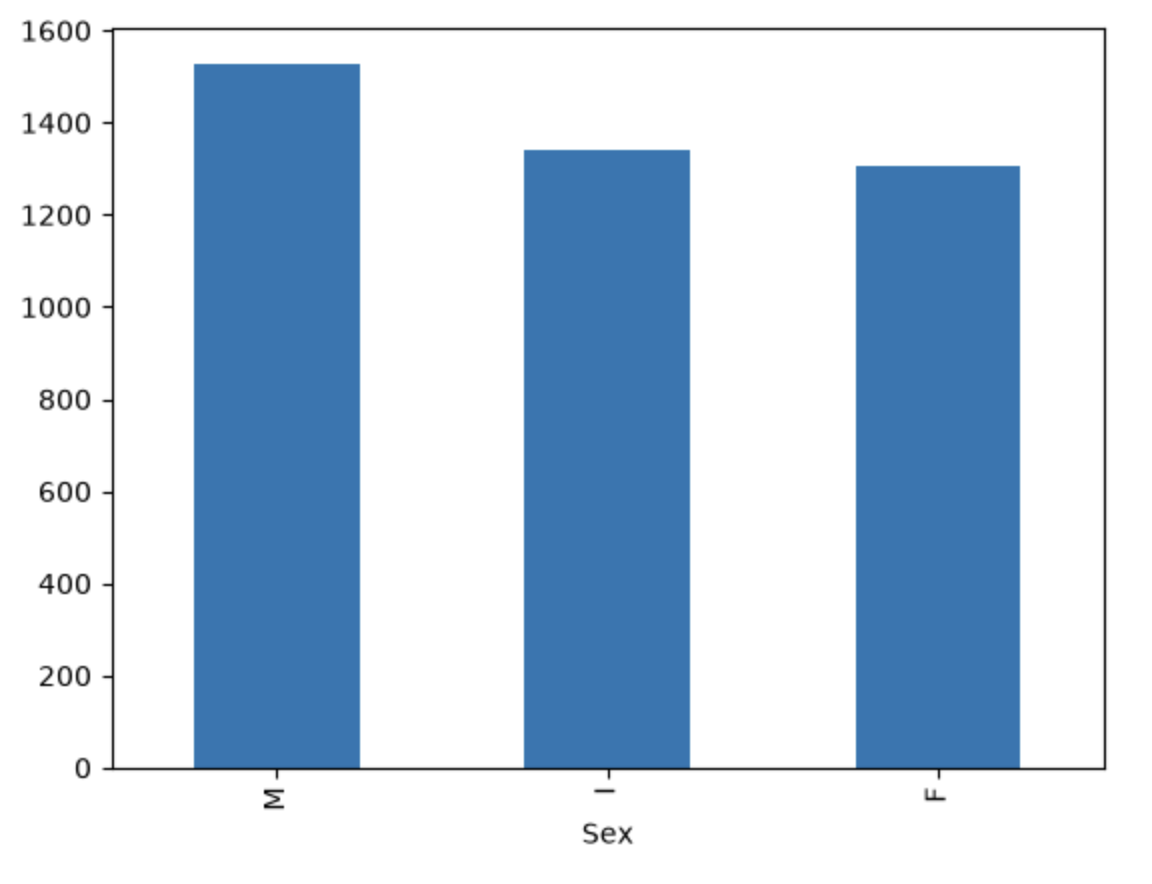
\includegraphics[width=10cm]{sex_distribution.png}\\
Sex Distribution

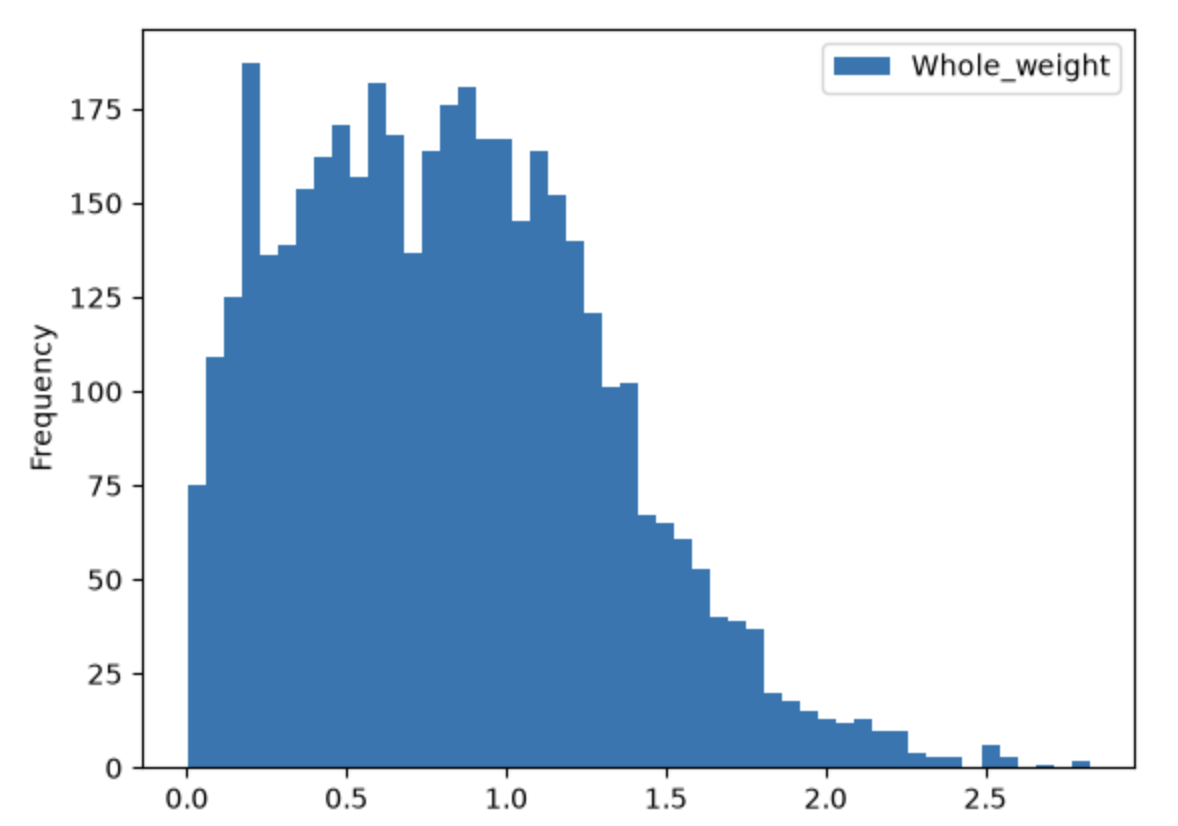
\includegraphics[width=10cm]{whole_weight_distribution.png}\\
Whole Weight Distribution

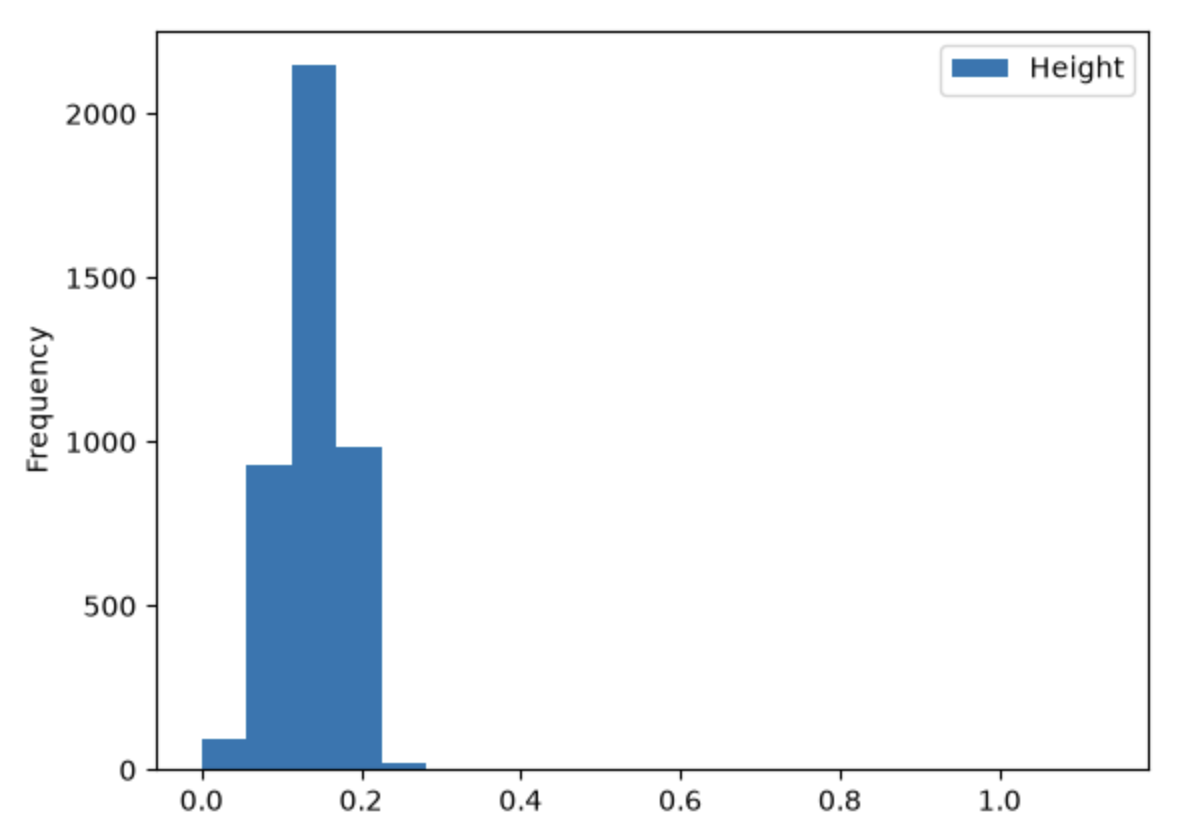
\includegraphics[width=10cm]{height_distribution.png}\\
Height distribution\vspace{0.5cm}\\

There are some issues with this data. It does not contain any environmental data, so some abalone may have different growth rates (or different rates in different dimensions) due to adverse (or unusually good) conditions.
We also do not know if it is data from abalone from a specific area or around the world, so we do not know how representative the data is. This ties into the previous point about environmental data. 
It is also from 1994, so it is somewhat old. This may matter if climate change has impacted abalone habitat conditions enough to impact their growth to age ratio.
Most relevantly, it does not specifiy which species of abalone the data is taken from, or even if it contains data from multiple species. This makes it difficult to say where this model could be used.\\
 
\section{Responsible AI/ML use}
In the context of this project, risks associated include breaking the license of the dataset. Since it is under the creative commons license, all that is required is to cite the authors as done here. 
The data in this set has no identifying information on any people or any private data, so there are no concerns about privacy.
Furthermore, the predictions are not relevant to any work which will affect people (e.g. no hiring decisions or insurance claims). 

\section{Models Used}
The baseline used is scikit-learn's DummyRegressor with the mean strategy (it always predicts the mean of the training set). The two trained models models used are ridge regression (using the scikit-learn Ridge model) and a k nearest neighbours model (using the scikit-learn KNeighborsRegressor model).\\

Ridge was chosen because the data seems to suit a linear model. In general, if an abalone is larger or heavier one would assume it is typically older, and if it is an infant it is younger. Ridge was chosen over lasso, as all features are suspected to be relevant. \\   

K nearest neighbours was chosen to have a non-linear model, as the dataset analysis showed that the data is not perfectly linear (oldest abalones were not the largest in any variable).\\

Originally, a decision tree model was proposed rather than a k nearest neighbour model. However, once implemented, I realised that the tree model collapsed into a linear model very early on. Since this does not deliver any interesting differences to look at (and thus learn from), I decided to switch to a k nearest neighbour model instead.

\section{Data Preparation and Tuning Process}
The data was split into 80\% train, 20\% test. A random split was deemed appropriate, since the rows are all independent (each is a separate abalone's measurements).
Different seeds for the random split were empirically tested and it was determined that the models behave similarly for different partitions and shuffles of the dataset.\\
A preprocessing pipeline was created to encode sex data and ignore all other data. This was done with one-hot encoding (as to not confuse the K nearest neighbours model with artifically imposed ordering), dropping one value as to not introduce collinearity.
No scaling was done for the K nearest neighbours model, as all features are alreay in the range 0-3 due to scaling being pre-performed on the dataset.

The errors chosen to measure performance are the r squared error (abbreviated as r2), root mean squared error (abbreviated as rms), and mean absolute error (abbreviated as mae).

No tuning was performed on the baseline. Both the ridge and the K nearest neighbour model were trained with GridSearchCV searching a parameter grid for the best parameters. Different numbers of folds were attempted empirically and delivered similar results. 
They were each trained separately with the penalty on each error (r2, rms, and mae) to see if different parameters were chosen. 
If different parameters were chosen for different penalties, the other error scores were inspected and the best overall parameters were chosen. 

Final settings:\\
Baseline: DummyRegressor, strategy=mean\\
Ridge: alpha=1.0\\
KNN: KNeighborsRegressor, algorithm=brute, metric=euclidean, n\_neighbors=15, weights=distance\\

\section{Error Analysis}
The root mean squared error is more sensitive to larger errors than the mean absolute error. They both represent the average error in prediction, just calculated in different ways. A smaller average error is indicative of a better model. 
The r2 error represents how much the model explains/handles variance. A perfect r2 score would be 1.\\
In this use case, neither false positives or false negatives have a substantially larger relevance (since this is not a situation such as predicting health conditions), so we do not need to put additional emphasis on reducing any particular sort of error over others.\\
Here is a table of the errors of each model.\vspace{0.5cm}\\
\begin{tabular}{|c|c|c|c|}
\hline
 model    & root mean squared error & mean absolute error & r2 error \\
\hline
 baseline & 3.298 & 2.467   & -0.001 \\
\hline
 ridge    & 2.249 & 1.592   & 0.534 \\
\hline
 k nearest neighbours      & 2.215 & 1.516   & 0.548 \\
\hline
\end{tabular}

The baseline has the largest root mean squared and mean absolute errors, and the smallest r2 error. Just based on error numbers, this indicates that the baseline has the worst performance among the models.\\
The ridge and k nearest neighbour models have very similar error results, with the k nearest neighbours being slightly better. \\

Calculated errors alone do not show the full picture though, so next we will analyse the residual graphs. A residual is the difference between the actual and the predicted value. The ideal residual is zero, which would indicate a perfect prediction.\\

    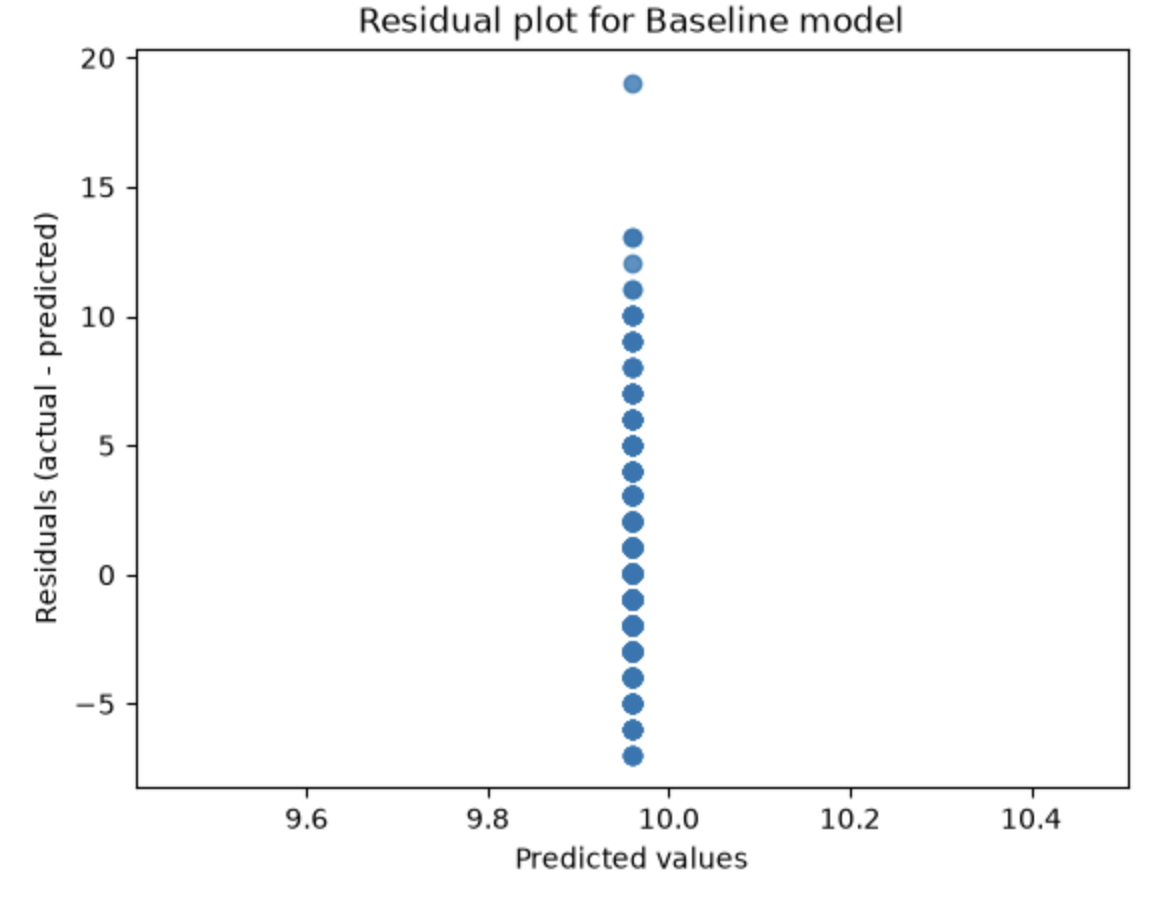
\includegraphics[width=10cm]{baseline_residuals.png}\\
This residual graph very clearly shows that the model always predicts the same value and is often wrong. It cannot predict other values, and is thus not very good. 

    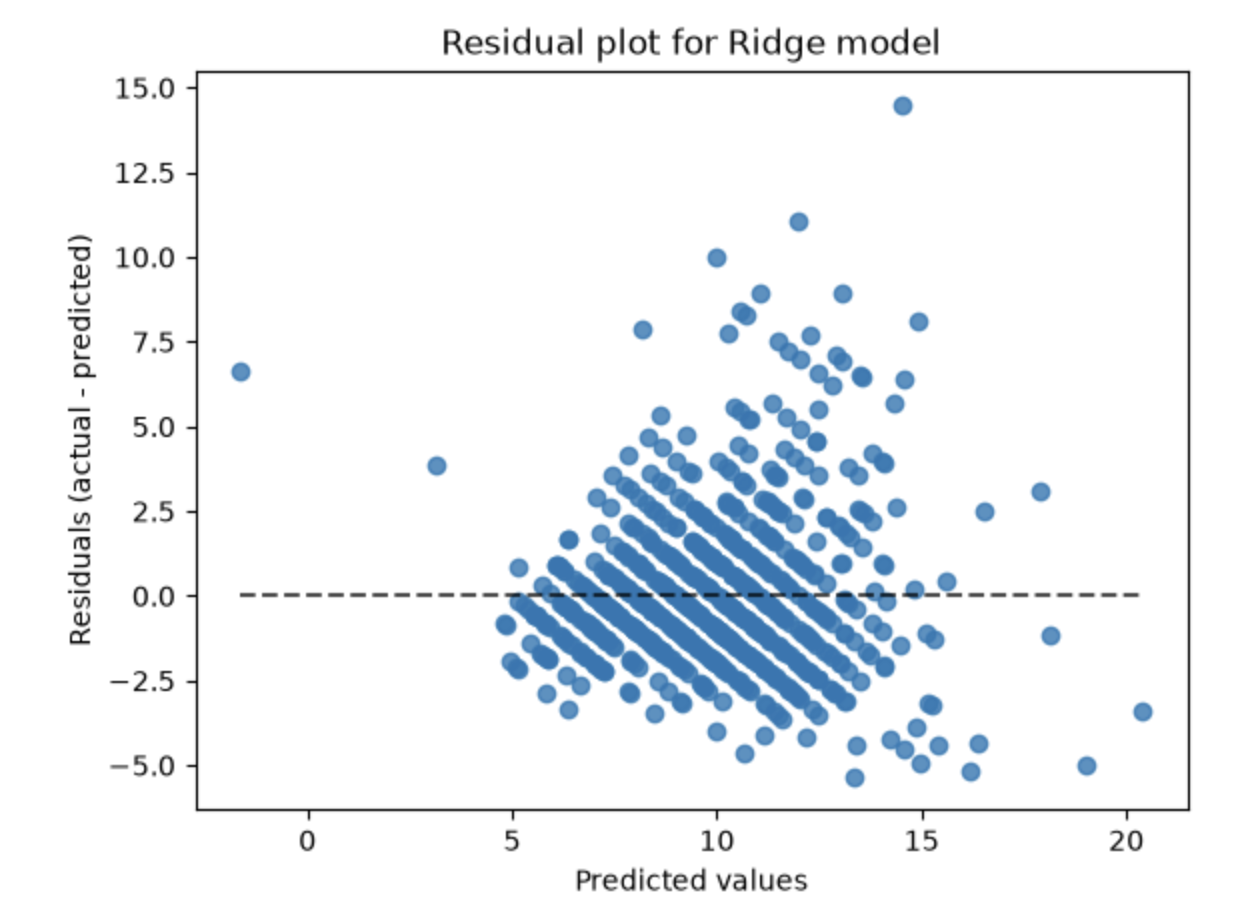
\includegraphics[width=10cm]{ridge_residuals.png}\\
The ridge model seems to mostly predict values between 5 and 15, thus having higher residual values when the true value does not lie in that interval.
We can see two particularly noticeable outliers, one where the model predicted near zero and one where the residual is near 15. When looking at the distribution of the target data there are a few values near 30, much higher than the average value, so this is likely one of these large outliers.

    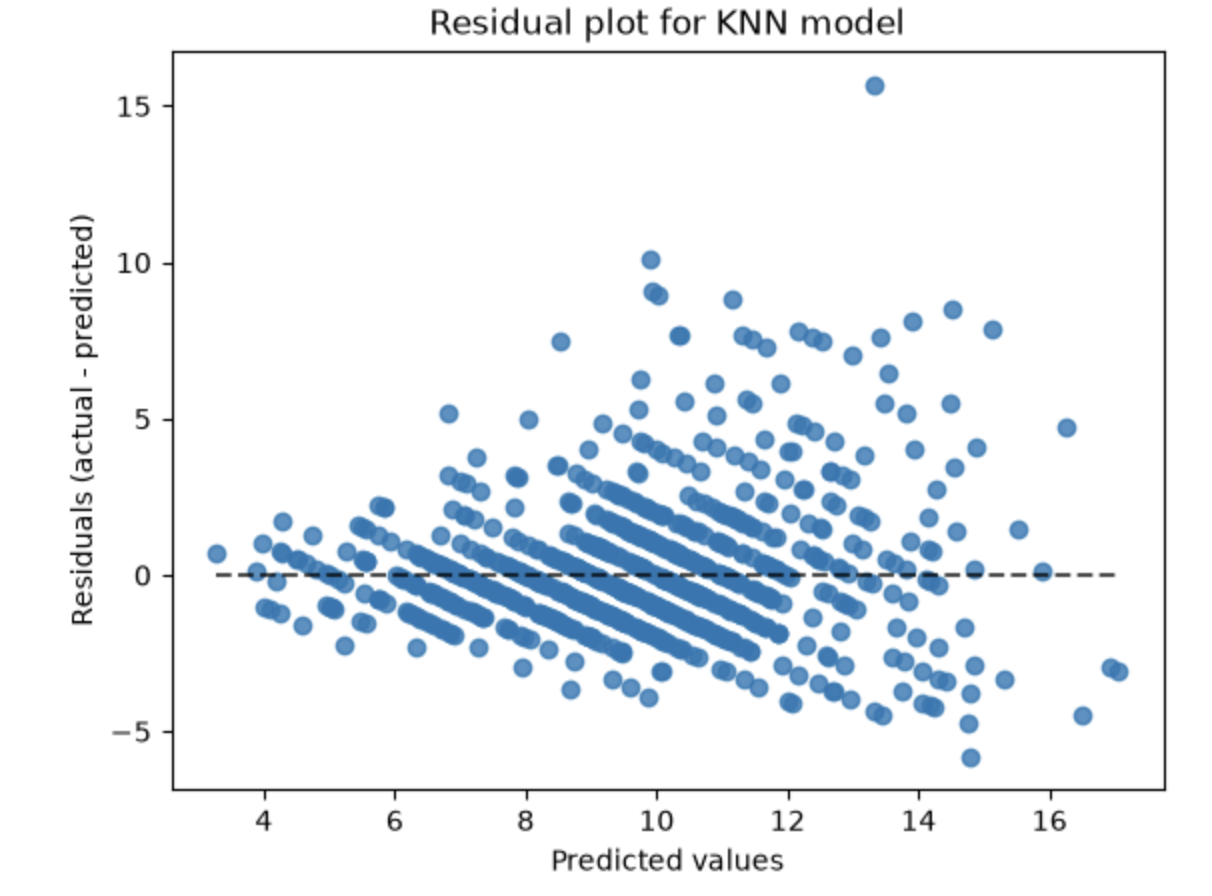
\includegraphics[width=10cm]{knn_residuals.png}\\
The k nearest neighbours model’s residual plot is more spread out and generally closer to the zero line than the ridge one. 
Much like the ridge model, there is one outlier where the residual was near 15. It is plausible this is also one of the very old specimens. 
The model seems to perform worse with larger target values, as can be seen by there being larger residuals for higher predicted values. It only predicts values between four and sixteen, which is a smaller interval than the ridge model. 

The low ability to predict high target values in both the ridge and the k nearest neighbours model indicates that they were not exposed to many high target features in training. This is likely because there are very few high target value features compared to lower values (the most common being ten).

\section{Final Results}
The current best performing model is the k nearest neighbours model with parameters algorithm=brute, metric=euclidean, n\_neighbors=15, and weights=distance.

We can determine this based on its error scores and the residual plot. The k nearest neighbours model has the lowest root mean squared error and the lowest mean absolute error. In terms of r2 error, the k nearest neightbours model is the highest. 
Based on comparing the residual plots (more analysis above), we can determine that the k nearest neighbours  model is better than the ridge model for the most common range of target values. 

However, the k nearest neighbours model is not very good at predicting high target values, as can be seen from the residual plot. This is because these values are rare, and thus the model does not know how to adapt to them.
Furthermore, the k nearest neighbours model is more resource intensive than the ridge model, so depending on the use case a slightly lower performance, cheaper model may be more appropriate.
Both the k nearest neighbours model and the ridge model are certainly much better than the baseline.

It is unclear exactly for which use cases this model is appropriate, as it is unknown which species of abalone the dataset covers. 
It would be useful for research, for instance when estimating the general age range of an abalone population in an area. 

The workflow, especially data preparation, was fairly simple and streamlined. It could potentially be improved upon, but its current state delivers satisfactory results.

\section{Limitations}
One major limitation in this portfolio was time constraints. If given more time, exploring more different models or more preprocessing (e.g. feature reduction) could have been interesting. Additionally, the quality of the model is limited due to above explained issues with the dataset (for instance, it does not include any environmental data).  

\section{Conclusion}
This report has covered the process and results of the machine learning portfolio assignment. The dataset, its preprocessing, the models used, results, and error analysis. The best model was the K nearest neighbours model, contradicting the hypothesis that the data had a linear structure. \\
It however, is not very good at estimating edge cases (i.e. unsually large and unusally small target values) and could be further improved, potentially with feature reduction or bootsrapping to include more edge case values in the training set. Developing a model which is more sensitive to outliers and aggregating them could also be an option.
Due to the lack of specificity of the data (it is unknown which species the data covers), the usefulness of the model is highly limited. As such, I would not recommend deploying it at this time. 

\begin{thebibliography}{999}

\bibitem{abalone}
  Nash, W., Sellers, T., Talbot, S., Cawthorn, A., \& Ford, W. (1994). 
  Abalone [Dataset]. UCI Machine Learning Repository. https://doi.org/10.24432/C55C7W.
\end{thebibliography}
\end{document}
